\section{SDL Models}
\label{sdl-sec:models}

Bearing that Knowles’ definition of \gls{SDL} occupies a prominent position in literature, it is usual to see \gls{SDL} as a process. Thus, different proposed models represent the understanding of the \gls{SDL} process and its constituent parts. \citeauthoronline{merriam:2007} (\citeyear{merriam:2007}, p.~110) classify these models into three types: linear, interactive, and instructional. For the \gls{Ph.D.} research purposes, I will present in more detail the linear (Section \ref{sdl-models-ss:linear}) and instructional (Section \ref{sdl-models-ss:instructional}) ones. The model type indicates how a pedagogical approach can embody the \gls{SDL} goals.

\subsection{Linear Models}
\label{sdl-models-ss:linear}

The first proposed models to \gls{SDL} had this characteristic: linearity. It is possible that the early authors did not believe strictly in this way. But, due to the inexistence of previous references, I think it is natural to propose a first minimum scaffold to refine it in the future. In this way, it does not seem to me as a helpful comprehension that these authors are “naive” when they propose their models. They give the first steps towards a better understanding and deepening \gls{SDL} as a process.

I list two prominent representatives of linear models: Allen Tough and Malcolm Knowles. I will discuss Knowles’ description of \gls{SDL} as a process in more detail. From Knowles' definition and my schema presented in Figure \ref{fig:sdl-process}, it is possible to identify five phases: (i) diagnosing learning needs, (ii) formulating learning goals, (iii) identifying human and material resources for learning, (iv) choosing and implementing appropriate learning strategies, and (iv) evaluating learning outcomes. Although it is not present in the literal definition, Knowles (\citeyear{knowles:1975}, p.~9, 29, 60) also adopts a preliminary phase called “setting a climate”. Thus, it is possible to see Knowles' model as composed of six phases instead of five.

We can compare the \gls{SDL} linear models to the first software lifecycle models. The waterfall model \cite[p.~8]{ruparelia:2010} also proposes a well-established sequence of phases that may invoke feedback loops. I believe that both Tough and Knowles considered other variables like internal dispositions or social context of the learner and judged them necessary during the \gls{SDL} process. However, these variables were not explicitly expressed in their proposed models. I list in Table \ref{tbl:sdl-competencies} all competencies proposed by Knowles (\citeyear{knowles:1975}, p.~61) to be used by self-directed learners as a self-rating instrument.

\begin{table}[ht]
\caption{List of \acrshort{SDL} competencies proposed for a self-rating instrument.}
\label{tbl:sdl-competencies}
\centering
\rowcolors{1}{}{lightgray}
\begin{tabular}{p{0.5cm}p{14.5cm}}
\hline
\multicolumn{2}{c}{\textbf{Competencies of Self-Directed Learning}} \\
\hline     
1 &
An understanding of the differences in assumptions about learners and the skills required for learning under teacher-directed learning and self-directed learning, and the ability to explain these differences to others.\\
2 &
A concept of myself as being a non-dependent and a self-directing person.\\
3 &
The ability to relate to peers collaboratively, to see them as resources for diagnosing needs, planning my learning, and learning; and to give help to them and receive help from them.\\
4 &
The ability to diagnose my own learning needs realistically, with help from teachers and peers.\\
5 &
The ability to translate learning needs into learning objectives in a form that makes it possible for their accomplishment to be assessed.\\
6 &
The ability to relate to teachers as facilitators, helpers, or consultants, and to take the initiative in making use of their resources.\\
7 &
The ability to identify human and material resources appropriate to different kinds of learning objectives.\\
8 &
The ability to select effective strategies for making use of learning resources and to perform these strategies skillfully and with initiative.\\
9 &
The ability to collect and validate evidence of the accomplishment of various kinds of learning objectives.\\
\hline

\end{tabular}

  \par\medskip\ABNTEXfontereduzida\selectfont\textbf{Source:} Adapted from \cite[p.~61]{knowles:1975}. \par\medskip
\end{table}

There are two main critiques of this type of model. First, the linearity can lead the learner or facilitator to admit this sequence as a strict and irrevocable flux to follow, precluding necessary returns to early phases to guarantee effective learning. Second, the simplicity of these models does not explicitly address other internal dimensions of the learner beyond the cognitive or meta-cognitive aspects (e.g., feelings) or external dimensions like structural barriers (e.g., racism, poverty). 

% \subsection{Interactive Models}
% \label{sdl-models-ss:interactive}

% \fbox{
%     \begin{minipage}[htb]{0.9\textwidth}
%         \vspace{0.3cm}
                
%         \colorbox{gray!30}{% create a colored box
%             \makebox[0.975\textrefers][l]{% center the text on the page
%                 \ \ \textbf{Further Writing}
%             }
%         }

%         \vspace{0.1cm}
        
%         \begin{itemize}
%             \item Presenting the main characteristics of interactive models.
%             \item Pointing out their limitations.

%         \end{itemize}

%         \vspace{0.25cm}
        
%     \end{minipage}
% }


\subsection{Instructional Models}
\label{sdl-models-ss:instructional}

The last class of \gls{SDL} models refers to frameworks that teachers can utilize in order to foster \gls{SDL} competencies into their programs and activities. I will present the \gls{SSDL} Model that “suggests how teachers can actively equip students to become more self-directed in their learning” \cite[p.~126]{grow:1991}. To achieve this, an axis (ranging from an Authority/Coach to a Consultant /Delegator teacher) situates what standing should be adopted in each situation (Table \ref{tbl:ssdl-model}).

% \fbox{
%     \begin{minipage}[htb]{0.9\textwidth}
%         \vspace{0.3cm}
                
%         \colorbox{gray!30}{% create a colored box
%             \makebox[0.975\textwidth][l]{% center the text on the page
%                 \ \ \textbf{Further Writing}
%             }
%         }

%         \vspace{0.1cm}
        
%         \begin{itemize}
%             \item Presenting the main characteristics of instructional models.
%             \item Describing in more detail the \gls{SSDL} Model (Table \ref{tbl:ssdl-model}) that “suggests how teachers can actively equip students to become more self-directed in their learning” \cite[p.~126]{grow:1991}.
%             \item Scrutinizing both the teacher and students’ stages (Figure \ref{fig:ssdl-matrix}).
%             \item Indicating that this work uses a combination of \citeauthoronline{knowles:1975}’ and \citeauthoronline{grow:1991}'s models.
%             \item Linking to the next section (challenges in \gls{SDL}).
%             \item Listing some limitations.

%         \end{itemize}

%         \vspace{0.25cm}
        
%     \end{minipage}
% }

\begin{table}[ht]
\caption{Staged \acrshort{SDL} Model structured into a table.}
\label{tbl:ssdl-model}
\centering
\rowcolors{1}{}{lightgray}
\begin{tabular}{
    >{\centering\arraybackslash}p{1.5cm}
    >{\centering\arraybackslash}p{3cm}
    >{\centering\arraybackslash}p{2cm}
    p{5.5cm}
}
\hline
\multicolumn{1}{c}{
    \textbf{Stage}
} &
\multicolumn{1}{c}{
    \textbf{Student}
} &
\multicolumn{1}{c}{
    \textbf{Teacher}
} &
\multicolumn{1}{c}{
    \textbf{Examples}
} \\
\hline     
Stage 1 &
Dependent &
Authority Coach &
Coaching with immediate feedback. Drill. Informational lecture. Overcoming deficiencies and resistance.\\
Stage 2 &
Interested &
Motivator, guide &
Inspiring lecture plus guided discussion. Goal-setting and learning strategies.\\
Stage 3 &
Involved &
Facilitator &
Discussion facilitated by teacher who participates as equal. Seminar. Group projects.\\
Stage 4 &
Self-directed &
Consultant, delegator &
Internship, dissertation, individual work or self-directed study-group.\\
\hline

\end{tabular}

  \par\medskip\ABNTEXfontereduzida\selectfont\textbf{Source:} Adapted from \cite{grow:1991}. \par\medskip
\end{table}

\citeauthoronline{grow:1991}'s model also signals how would be a desirable matching between student \gls{SDL} stage and teacher standing. Figure \ref{fig:ssdl-matrix} shows a confusion matrix, highlighting that it should exist a dynamic in our educational practices aiming to materialize \gls{SDL} of our students. In this research, I adopt a combination of \citeauthoronline{knowles:1975}’ and \citeauthoronline{grow:1991}'s models, providing the constructs for the discussion of results.

\begin{figure}[ht!]
\centering

\caption{\textmd{Staged \acrshort{SDL} Model structured from a confusion matrix.}}
\label{fig:ssdl-matrix}
\fcolorbox{gray}{white}{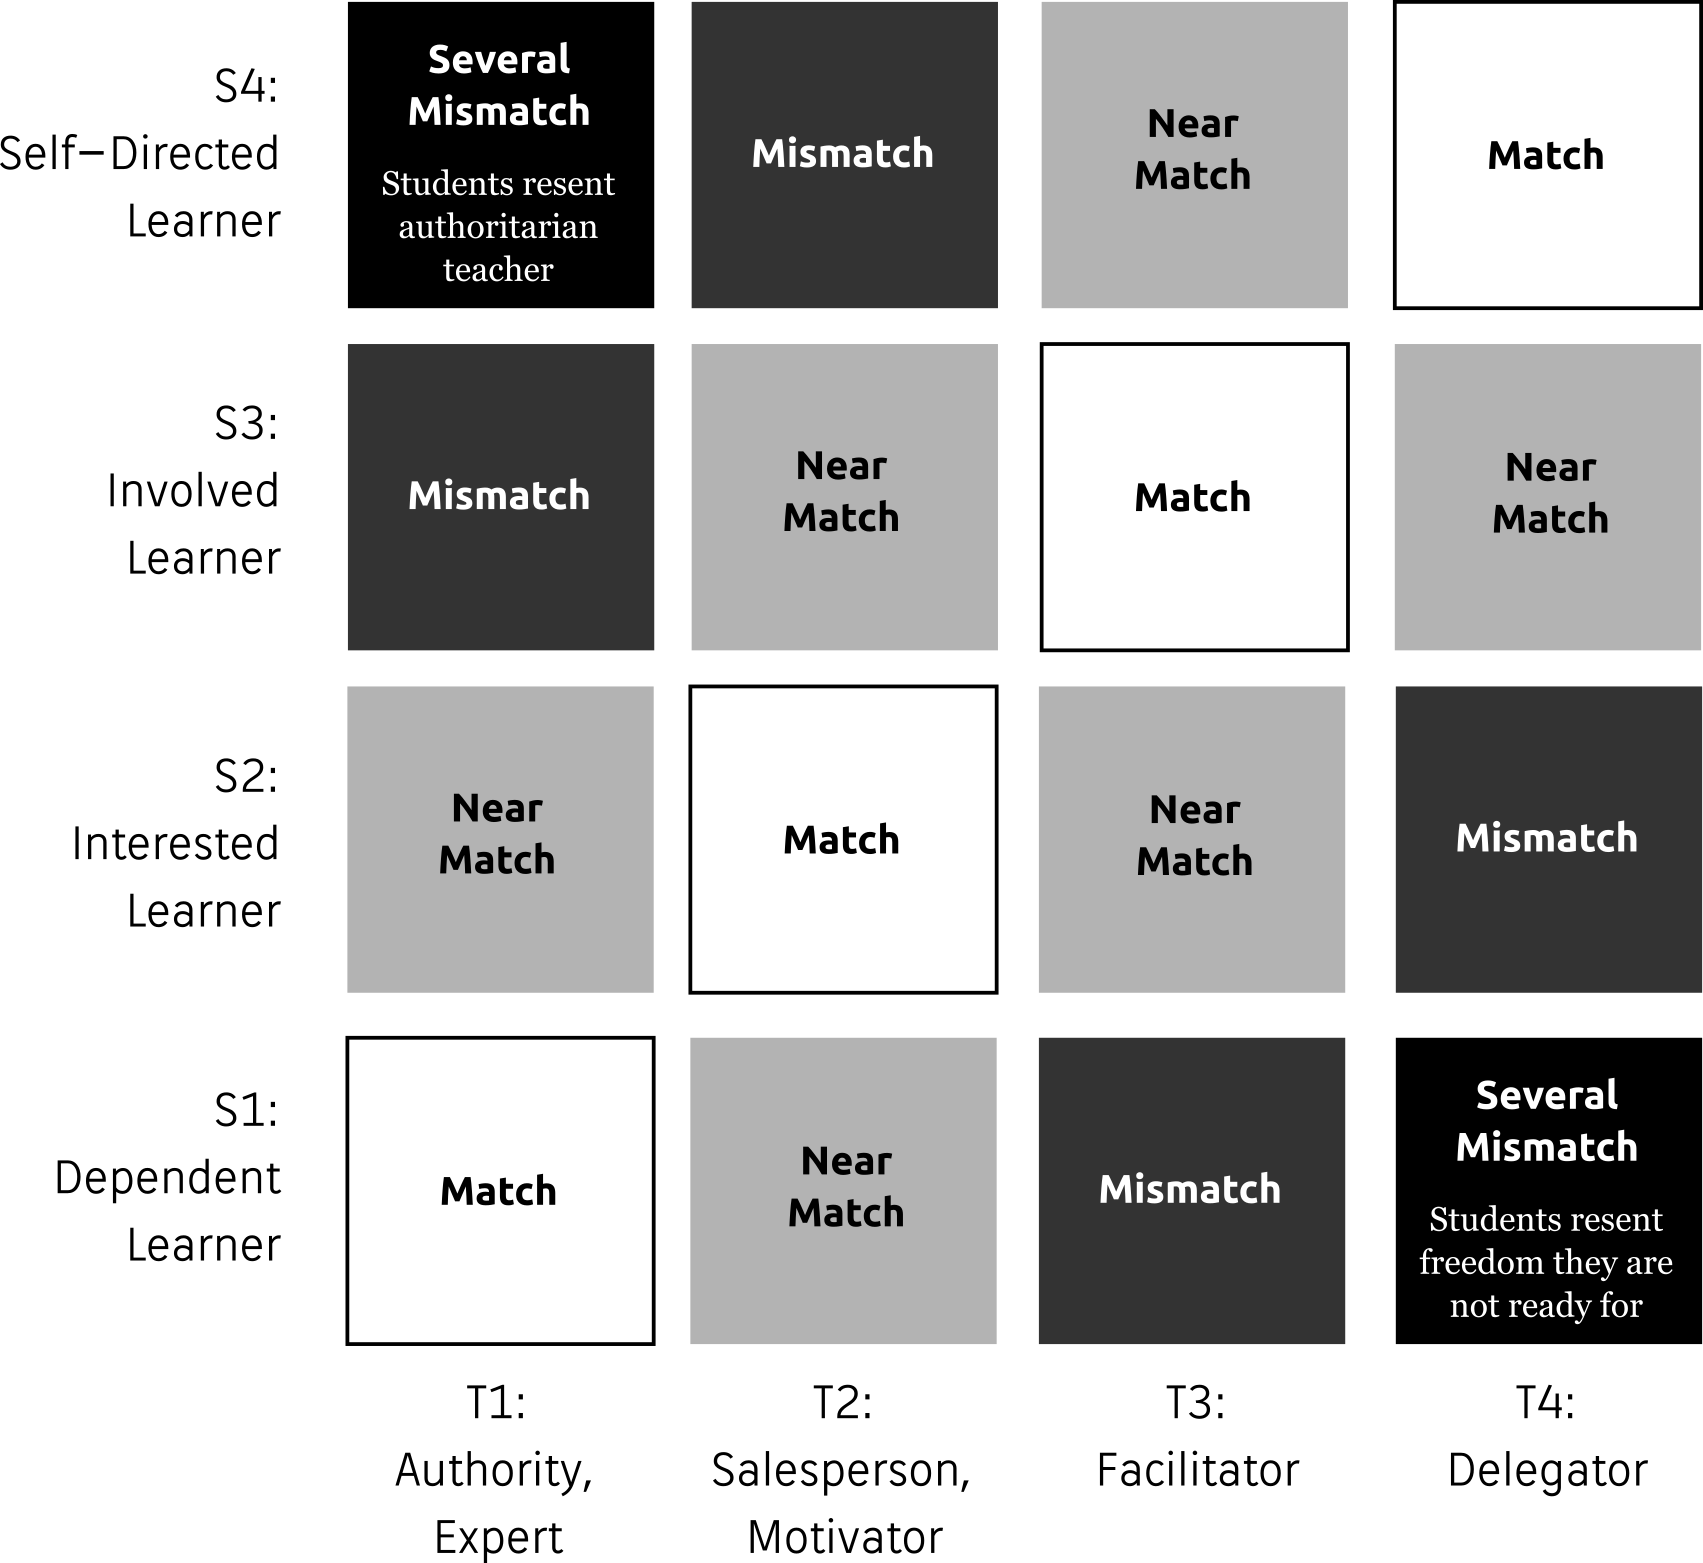
\includegraphics[width=0.9\textwidth]{images/chapter-02/grow.png}}

\par\medskip\ABNTEXfontereduzida\selectfont\textbf{Source:} Adapted from \cite{grow:1991}.%\citeauthor{manualufpe2020} (\citeyear{manualufpe2020}) \par\medskip
\end{figure}